\documentclass{article}

\usepackage[]{amsmath} 
\usepackage[]{amsthm} 
\usepackage[]{amssymb} 
\usepackage[]{microtype}
\usepackage[]{mathtools} 
\mathtoolsset{centercolon}
\usepackage[]{graphicx} 
\usepackage[]{subcaption} 

% code listings
\usepackage[]{listings} 
\usepackage[usenames, dvipsnames, svgnames, table]{xcolor} 
\usepackage[]{mdframed} 
\usepackage[]{calc} 
\usepackage[]{fontspec} 

\newfontfamily\monocode[BoldFont=Source Code Pro]{Source Code Pro Light}
\newfontfamily\latocode[Numbers=OldStyle, BoldFont=Lato Regular]{Lato Light}

\definecolor{TMgreen}{RGB}{14, 191, 48}
\definecolor{TMorange}{RGB}{243, 126, 25}
\definecolor{TMred}{RGB}{230, 6, 85}
\definecolor{TMcodeBackground}{RGB}{224, 224, 224}
\definecolor{TMcodeFrame}{RGB}{109, 108, 109}

\mdfdefinestyle{TMstyleCode}{
            skipabove=4mm,
            skipbelow=0mm,
            %remove borders
            rightline=false,
            topline=false,
            bottomline=false,
            linewidth=1mm,
            %margins
            innertopmargin=2mm,
            innerleftmargin=0mm,
            innerbottommargin=0mm,
            innerrightmargin=10pt,
            linecolor=TMcodeFrame,
            backgroundcolor=TMcodeBackground
}

\lstdefinestyle{TMstyle}{
    showstringspaces=false,
    numbers=left,
    numbersep=7mm,
    numberstyle=\color{Black}\latocode,
    stepnumber=1,
    tabsize=3,
    breakatwhitespace=false,
    breaklines=true,
    captionpos=b,
    basicstyle=\color{Black}\monocode,
    commentstyle=\color{TMgreen}\latocode,
    keywordstyle=\color{TMorange}\bfseries\latocode,
    stringstyle=\color{TMred}\latocode,
    frame=leftline,
    framesep=0mm,
    xleftmargin=3mm,
    framesep=2mm,
    framerule=0mm,
    abovecaptionskip=5mm,
    aboveskip=\baselineskip,
    belowskip=\baselineskip
}

% need to use inner commands to avoid the verbatim nature
% of listing environments!

\lstnewenvironment{TMcode}[3]
{
    \lstset{style=TMstyle, language=#1, caption=#2}
    \mdfsetup{style=TMstyleCode}
    \mdframed
    \hspace*{3mm}
    \minipage{0.75cm}
    \includegraphics[width=\linewidth]{images/code2.png}
    \endminipage
    \hspace*{1mm}
    \minipage{\textwidth-1.05cm}
        {\latocode\Large #3}
    \endminipage
    \vspace*{-2mm}
}
{
    \endmdframed
}
\title{\textsc{MATINF4160 Fall 2016 \\
Mandatory Assignment 3}}
\date{\small\textbf{Due: November 17th, 2016}}
\author{Ivar Haugal{\o}kken Stangeby}
\renewcommand{\bf}[1]{\mathbf{#1}}

\begin{document}
   \maketitle 

   \section*{Problem 1}
   \label{sec:problem_1}
    
   We wish to find control points $\bf{c}_0, \ldots, \bf{c}_5$ such that the
   B\'ezier curve
   \begin{equation}
       \notag
       \bf{p}(t) = \sum^{5}_{j=0} \bf{c}_j B_j^n(u)
   \end{equation}
   interpolates a given function $\bf{f}$ and its $i$th derivatives in the
   points $a$ and $b$ for $i = 0, 1, 2$. That is, we want $\bf{p}^{(i)}(a) =
   \bf{f}^{(i)}(a)$ for $i = 0, 1, 2$. We have in general that the control
   points $\bf{c}_j$ can be found by the following two formulas:
   \begin{align*}
       \bf{c}_j = \sum^{i}_{j=0} {i \choose j} \bf{b}_j, 
    && \bf{c}_{n-i} = \sum^{i}_{j=0} (-1)^j {i \choose j} \bf{b}_{n-j}
   \end{align*} 
   where we define
   \begin{align*}
       \bf{b}_i &\coloneqq \frac{(n - i)!}{n!} (b-a)^i \bf{f}^{(i)}(a), \\
       \intertext{for the leftmost control points, and define}
       \bf{b}_{n-i} &\coloneqq \frac{(n - i)!}{n!} (b-a)^i \bf{f}^{(i)}(b).
   \end{align*}
   for the rightmost control points. We start by computing the $\bf{b}_i$ and
   $\bf{b}_{n-1}$. This yields
   \begin{align*}
       \bf{b}_0 &=  f(a) & \bf{b}_1 &= \frac{1}{5}(b-a)\bf{f}'(a) \\
       \bf{b}_2 &=  \frac{1}{20}(b-a)^2\bf{f}''(a) & \bf{b}_3 &= \frac{1}{20}(b-a)^2\bf{f}''(b) \\
       \bf{b}_4 &=  \frac{1}{5}(b-a)\bf{f}'(b) & \bf{b}_5 &= \bf{f}(b)
   \end{align*}
   It then follows that the control points are given by
   \begin{align*}
       \bf{c}_0 &=  \bf{b}_0 & \bf{c}_1 &= \bf{b}_0 + \bf{b}_1 \\
       \bf{c}_2 &=  \bf{b}_0 + 2\bf{b}_1 + \bf{b}_2 & \bf{c}_3 &= \bf{b}_5 - 2\bf{b}_4 + \bf{b}_3 \\
       \bf{c}_4 &=  \bf{b}_5 - \bf{b}_4 & \bf{c}_5 &= \bf{b}_5.
   \end{align*}
    
   \section*{Problem 2}
   \label{sec:problem_2}
   
    In this problem we consider an implementation of a $C^2$ cubic spline curve
    interpolation. We interpolate two data sets, $\bf{x}_i = (x_i, y_i)$ with 
    \begin{align*}
        (x_0, \ldots, x_9) &= (261, 261, 283, 287, 280, 281, 302, 319, 335, 277)\\
        (y_0, \ldots, y_9) &= (703,738, 718, 723, 735, 736, 731, 748, 737, 682)
    \end{align*}
    and $\bf{x}_i = (\cos(s_i), \sin(s_i))$ where
    \begin{equation}
        \notag
        (s_0, \ldots, s_{12}) = (0, 0.24, 0.39, 0.78, 1.03, 1.18, 1.56, 1.81, 1.96, 1.96, 2.34, 2.59, 2.74, 3.12).
    \end{equation}
    The general idea when looking for a Hermite spline interpolation is finding
    the suitable knot vector, where we want sufficient resolution where the $
    \bf{x}_i$ varies a lot. To each pair of data points we fit a cubic B\'ezier
    curve with control points tweaked for $C^2$ continuity. In this assignment
    we consider the parametrization
    \begin{equation}
        \notag
        t_{i+1} - t_i = \| \bf{x}_{i+1} - \bf{x}_i\|^\mu,
    \end{equation}
    for $\mu = 0, 0.5, 1$ and examine how it affects the interpolation. The
    interpolations can be computed and visualized with the following code:
    \begin{TMcode}{python}{spline\_interpolation.py}{Interpolating datasets}
from hermite_interpolation import *
import numpy as np

x_values = np.array([(261, 703), (261, 738),\
    (283, 718), (287, 723), (280, 735), \
    (281, 736), (302, 731), (319, 748),\
    (335, 737), (277, 682)])
   
for i, mu in enumerate([0, 0.5, 1]):
    curve = HermiteInterpolation(x_values,\
        order_of_continuity=2,\
        label='$\\mu = %0.2f$' % mu, mu=mu)
    curve.plot(display=True, filename='one_%d.pdf' % i)
\end{TMcode}

\begin{figure}
    \centering
    \label{fig:one}
    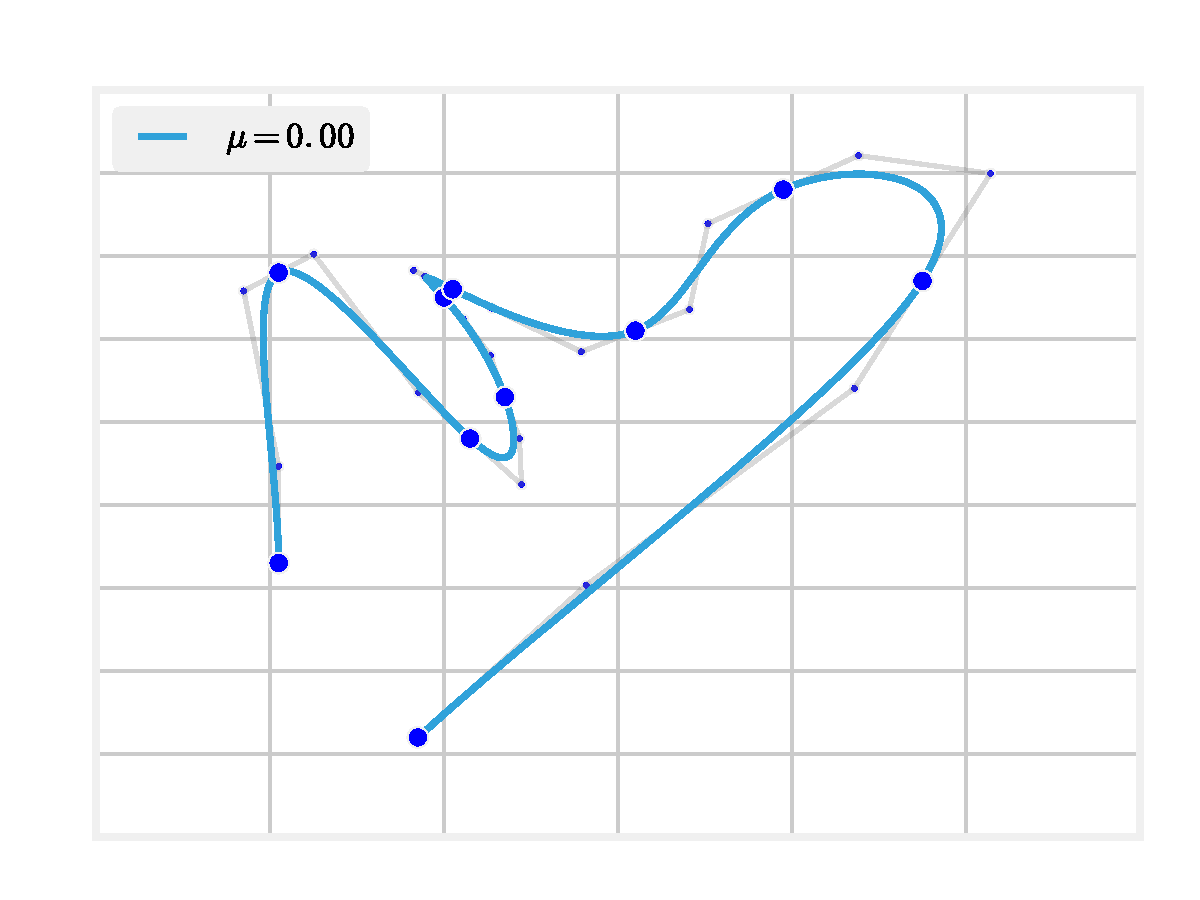
\includegraphics[scale=0.4]{pictures/one_0.pdf} 
    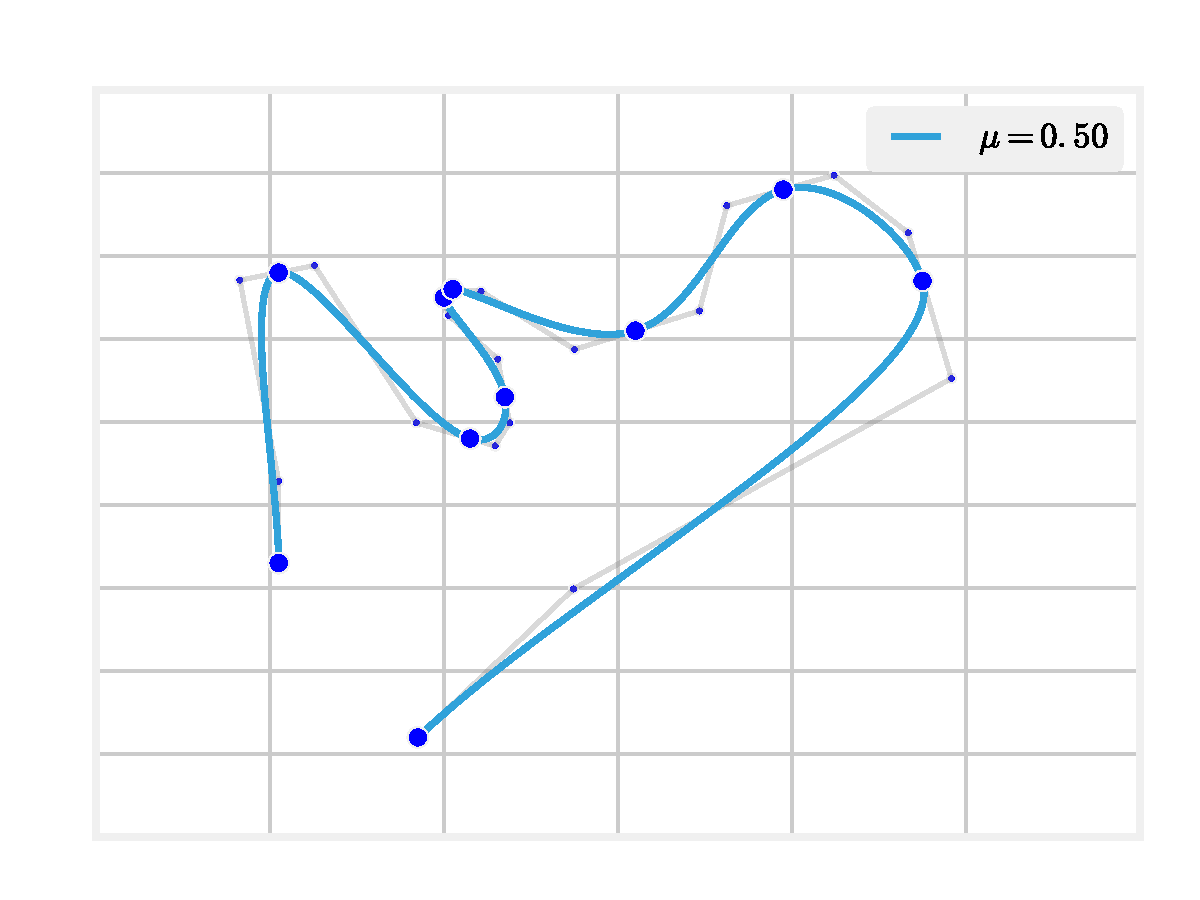
\includegraphics[scale=0.4]{pictures/one_1.pdf}
    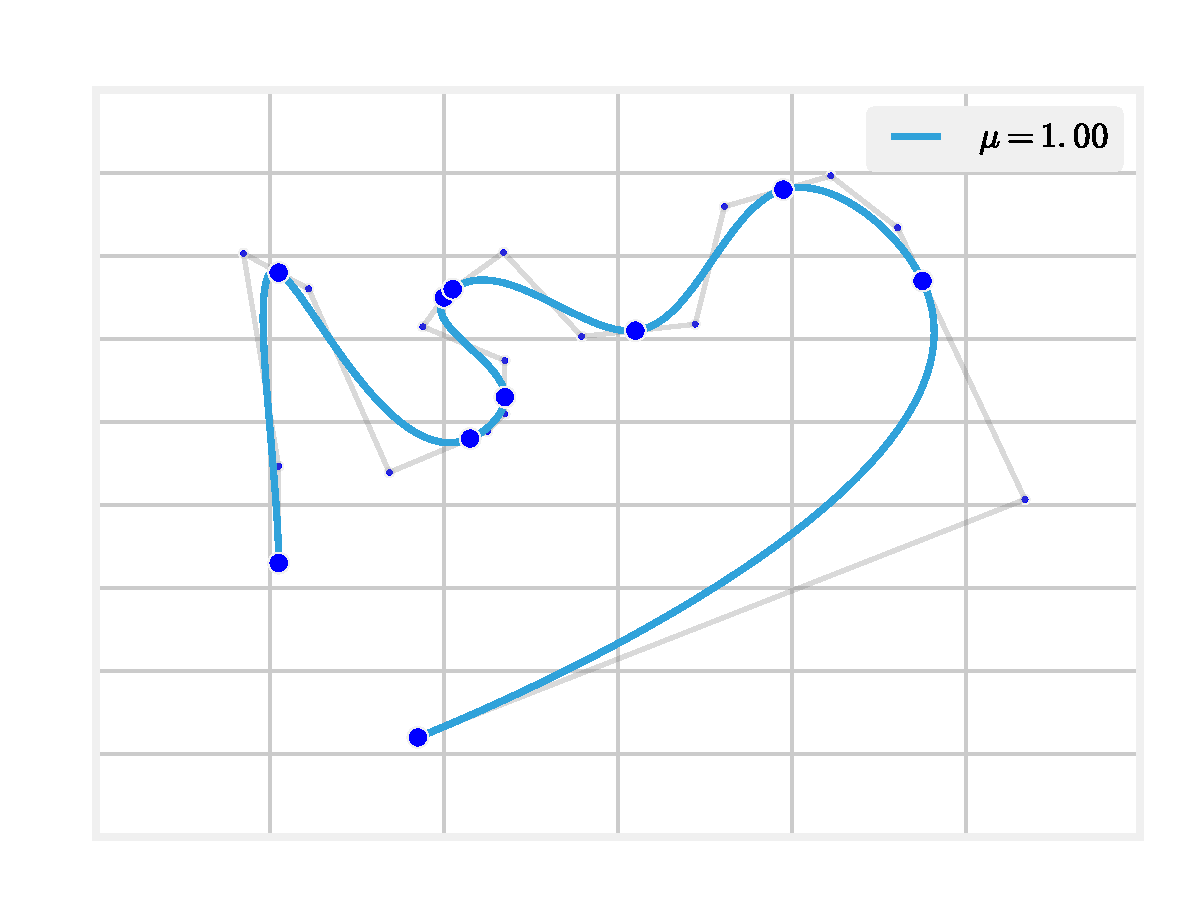
\includegraphics[scale=0.4]{pictures/one_2.pdf}
    \caption{The first dataset visualized for three different values of
    $\mu$. The interpolating curve is visualized in light blue, the large
    dark blue dots are the original data points.}
\end{figure}

\begin{figure}
    \centering
    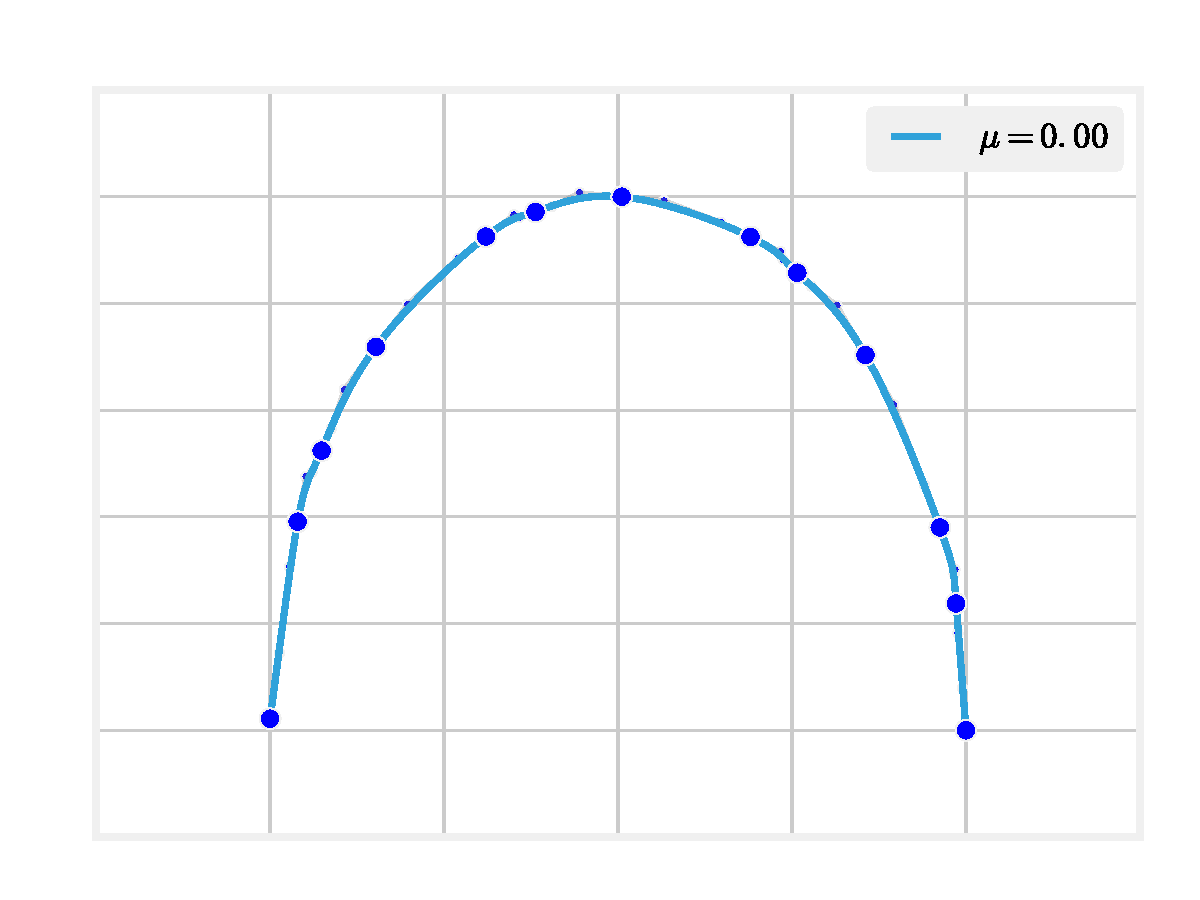
\includegraphics[scale=0.4]{pictures/two_0.pdf} 
    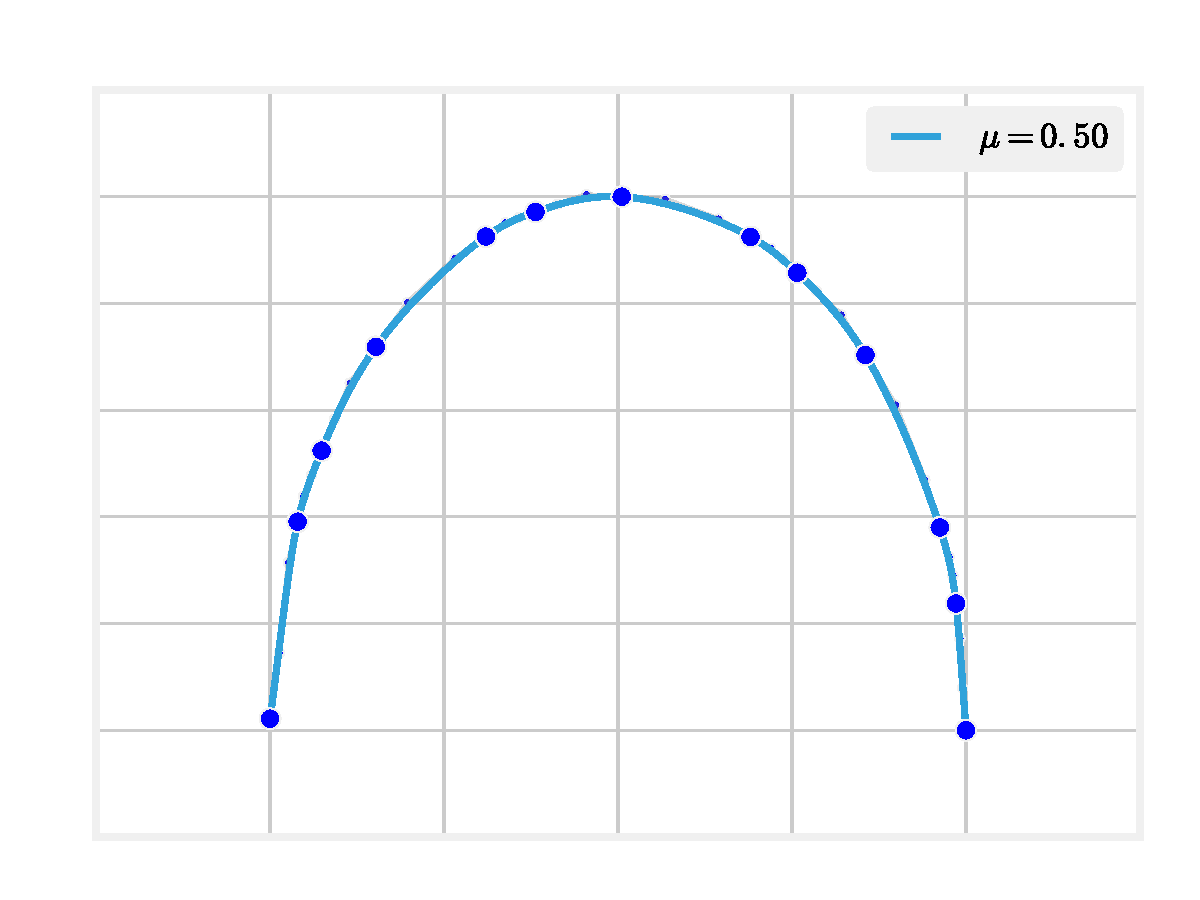
\includegraphics[scale=0.4]{pictures/two_1.pdf}
    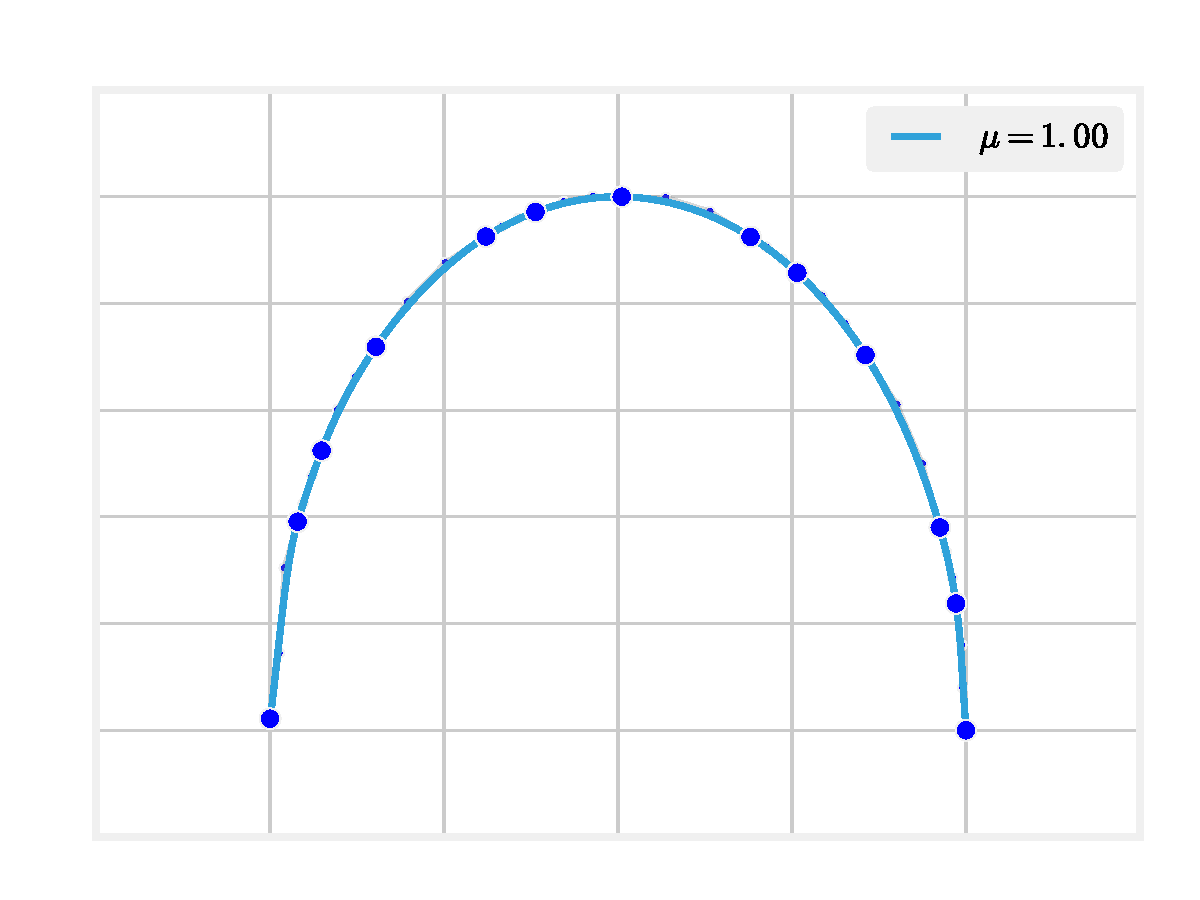
\includegraphics[scale=0.4]{pictures/two_2.pdf}
    \caption{The second dataset visualized for three different values of
    $\mu$. The interpolating curve is visualized in light blue, the large
    dark blue dots are the original data points.}
\end{figure}

\end{document}
